\chapter{Анализ механизмов движения мобильных плавающих роботов}\label{ch:ch1}

В данной главе представлен обзор существующих способов перемещения в жидкости. Рассмотрены прототипы водных роботов, приводимые в движение различными способами. 

\section{Введение}\label{sec:ch1/sec1}

В последние десятилетия активно развивается область по разработке мобильных роботов. В настоящее время уделяется существенное внимание разработке автономных мобильных роботов, предназначенных для решения определенных задач в разных средах. Появляющиеся роботы охватывают различные среды: роботы, перемещающиеся по твердой поверхности~\cite{Lozano_2012, Domel_2017, Kilin_et_al_2017, Bozek_2020}, роботы, перемещающиеся по воздуху~\cite{Kim_2008, Miller_2007}, водные роботы, перемещающиеся по поверхности жидкости~\cite{Pshihopov_2014, Moreira_2011}  и на глубине~\cite{Pshihopov_2014, Gornak_MMT3000, Matvienko_2017}. 

Среди водных роботов можно выделить надводные и подводные аппараты. Надводные роботы --- это роботы, работающие на поверхности воды. Из них наиболее интересная группа --- это автономные или полуавтономные суда-беспилотники. Автономные суда предполагают полностью безэкипажное перемещение, полуавтономные --- постоянно или некоторую часть времени управляются оператором (телеуправляемые суда).

Активное развитие подводных автономных аппаратов пришлось на 90-е годы XX века, что совпало с бурным развитием микроэлектроники и микропроцессорной техники, компьютерных и сенсорных технологий, созданием новых материалов. За несколько лет было разработано около 30 совершенно новых автономных необитаемых подводных аппаратов (АНПА) по всему миру~\cite{Yuh_2000}. В первое десятилетие XXI века в среднем появлялось до 70 новых проектов автономных подовдных аппаратов~\cite{Bocharov_2009}.

Для автономных водных роботов помимо конструкции важно разработать адекватную модель движения и систему управления. Навигационная система и система планирования траектории должны определять местоположение аппарата и движение по выбранному курсу~\cite{Fiorelli_2006, Lapierre_2007, Burdinskiy_2012}. При наличии датчиков или системы технического зрения нужно предусмотреть сохранение получаемой информации и дальнейшую ее обработку~\cite{Huster_2001, Dunbabin_2006}. В системах управления могут использоваться системы нечеткой логики и нейронные сети~\cite{Loebis_2004, Ishii_1995, Xiang_2017, Zhang_2008}.

В России в настоящее время одним из ведущих институтов работающих по данному направлению является Институт проблем морских технологий Дальневосточного отделения Российской академии наук (ИПМТ ДВО РАН)~\cite{Ageev, Kiselev_2012}. Сотрудниками института разрабатываются конструкции моделей АНПА~\cite{Boreyko_2011, Iznarcev_2007}, изучаются динамические характеристики~\cite{Kiselev_2012}, бортовые системы управления~\cite{Iznarcev_2005}, алгоритмы движения~\cite{Kiselev_2004}.



Развиваются области в создании роботов использующих как более традиционные способы перемещения, так и имеющие новые принципы приведения в движение. Отдельную область составляет исследование динамики водных роботов, имитирующих способы передвижения живых существ и роботов, не имеющих внешних подвижных элементов. Передвижение устройств без внешних подвижных элементов реализуется за счет движения внутренних масс и вращения роторов. Такие «экзотические» транспортные средства могут применяться в специфических (критических) условиях, например в условиях космоса или на больших глубинах.

Для построения модели движения аппаратов, движущихся в вязкой среде, используются законы гидродинамики, записанные в виде уравнений для действующих сил и моментов. В общем случае внешние силы можно разделить на силы, описывающие взаимодействие объекта с жидкостью, силы, обусловленные воздействием окружающей среды и движущие силы (тяговые силы). При описании движения различных типов роботов обычно вводят допущения об идеальности жидкости, совпадении главных осей инерции с осями симметрии тела.

Взаимодействие аппарата со средой описывается гидростатическими, гидродинамическими и управляющими силами и моментами. К гидростатическим относят остаточную плавучесть, которая описывает разницу между действительным запасом плавучести и расчётным и продольный и поперечный моменты остойчивости. Остойчивость определяет защищенность судна от опрокидывания, то есть способность противостоять внешним силам, пытающимся увеличить крен или дифферент. К гидродинамическим воздействиям относятся силы вязкого сопротивления и инерционные силы, зависящие от присоединенных масс жидкости. Гидродинамические силы также зависят от формы тела объекта и режима обтекания, который характеризуется числом Рейнольдса.

Силы, обусловленные воздействием окружающей среды включают в себя описание морских течений, волн и ветра.

Движущие силы возникают благодаря движителям аппарата, например, силы, возникающие вследствие вращения гребных винтов и силы действующие на поверхность рулей.

Одной из наиболее сложных задач является определение коэффициентов присоединенных масс, присоединенных моментов, моментов инерции тела. Для тел простой формы существуют ряд приемов вычисления данных параметров~\cite{Pantov_etc_1973}.

Силы вязкого сопротивления можно приближенно определить на стадии проектирования аппарата, используя численные методы расчета либо эмпирические зависимости, определяемые формой корпуса. В дальнейшем результаты уточняются при испытаниях реального аппарата в аэродинамической трубе и в опытовых бассейнах.

Выделим существующие способы перемещения в жидкости:

\begin{enumerate}
	\item Перемещение за счет использования гребных винтов.
	\item Перемещение за счет изменения формы тела.
	\item Перемещение за счет использования реактивного привода.
	\item Перемещение за счет действия внутренних механизмов.
\end{enumerate}

Рассмотрим подробнее каждый из этих способов.

\section{Перемещение за счет использования гребных винтов}\label{sec:ch1/sec2}

В настоящее время для водных мобильных систем, а также морских и речных судов, наиболее распространенным способом перемещения является перемещение с помощью гребных винтов. Способ перемещения с помощью винтов называют традиционным способом. Аппараты, используемые гребные винты широко используются для мониторинга и проведения различных операций. В частности, для мониторинга подводного рельефа и подводной геологоразведки, мониторинга обшивок подводных конструкций, проведение ремонтных работ на больших глубинах и в условиях химического или радиационного загрязнения и т.д. 

Гребные винты могут иметь от двух до шести лопастей, которые располагаются на равных угловых расстояниях друг от друга. Винты обычно размещаются за кормой судна и находятся на достаточной глубине. Повышение эффективности работы гребных винтов может осуществляться за счет применения судовых рулей и специальных направляющих устройств. На транспортном средстве может быть установлено один, два и более рулей, которые, как правило, располагаются за винтами~\cite{Basin_Anfimov_1961}. Таким образом может быть использована схема с гребным винтом и рулем. Существует вариант использования нескольких винтов, расположенных под разными углами~\cite{Lebedev_Pershits_1969, Gornak_MMT3000}

Теория управления транспортных средств, перемещающихся в жидкости за счет гребных винтов, хорошо изучена~\cite{Ageev, Fossen, Fossen2, Basin_Anfimov_1961, Lebedev_Pershits_1969}. В общем случае при криволинейном движении на объект действуют гидродинамические силы, распределенные по поверхности корпуса и рулей, сила полезной тяги, создаваемая движителями (винтами), а также, при движении по поверхности воды, сила давления ветра на надводную часть корпуса. Однако при описании движения вводятся некоторые допущения: транспортное средство рассматривается как твердое тело, которое движется в идеальной жидкости под действием внешних сил, к которым добавляются силы, возникающие вследствие вязкости жидкости.

Рассмотрим работы, в которых описаны конструкции автономных водных роботов, исследуются системы управления водными роботами, которые перемещаются за счет гребных винтов.

В работе~\cite{Gornak_MMT3000} описан автономный необитаемый подводный аппарат ММТ-3000, разработанный в Институте Проблем Морских Технологий ДВО РАН, г. Владивосток. В статье приведена структура аппарата и рассмотрены основные системы, входящие в его состав. Данный робот решает задачи широкого круга --- от морской биологии до геологических исследований. Глубина погружения аппарата --- 3000 метров. Имеется два типа конструкции движителей: два гребных винта на поворотных валах и три фиксированных гребных винта, расположенных под углом друг к другу. Описана система управления, которая способна обеспечивать движение робота в автономном режиме. Внешний вид аппарата ММТ-3000 представлен на рисунке~\ref{MTT3000}. 

\begin{figure}[h]
	\centering
	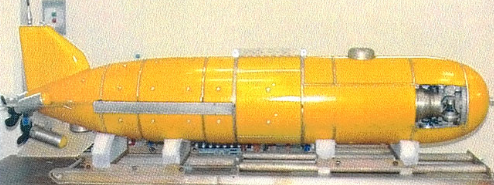
\includegraphics[width=0.7\linewidth]{MTT3000.png}%
	\caption{Автономный необитаемый подводный аппарат ММТ-3000}
	\label{MTT3000}
\end{figure}

Стоит отметить, что у Института Проблем Морских Технологий ДВО РАН огромный опыт по разработке водных роботов, существует множество работ, в которых описаны конструкции разработанных аппаратов, системы управления для них, рассмотрены задачи практического применения~\cite{Matvienko_2017, Naumov_2011, Boreyko_2011, Iznarcev_2007, Vaulin_2017, Inzarcev_2016}.

В работе~\cite{Pshihopov_2014} рассмотрена интеллектуальная система управления автономным подводным аппаратом. Планирование и управление движением построено на иерархической структуре. Подсистема планирования движения основана на нейросети и позволяет определять и обходить препятствия на пути движения робота. Система управления позволяет двигаться вдоль заданной траектории из точки в точку с заданной скоростью. В работе приводятся результаты моделирования системы управления. В качестве объекта моделирования выбран подводный аппарат, который приводится в движение гребным винтом и двумя подруливающими устройствами: горизонтальным и вертикальным. При этом гребной винт может менять свою ориентацию на некоторый угол в горизонтальной и вертикальной плоскости. Для моделирования положение центра масс и компоненты тензора инерции аппарата вычислены в пакете SolidWorks, гидродинамические характеристики расчитаны в программных комплексах FineHexa и STAR CD, присоединенные массы расчитаны по эмпирическим зависимостям в приближении формы аппарата эллипсом. В результате моделирования было показано, что интеллектуальная система управления позволяет избегать столкновений с подвижными и неподвижными препятствиями и способна выполнять поставленные задачи по движению робота по заданной траектории. На практике данная система управления была реализована на базе автономного надводного катера, и, в процессе испытаний, показала свою работоспособность при движении из одной точки в другую.



\subsection{Перемещение за счет изменения формы тела}\label{sec:ch1/sec3}

Хотя в разработке и исследовании движения кораблей и подводных лодок, перемещающихся за счет гребных винтов, были достигнуты значительные успехи, в настоящее время возник интерес к небольшим водным мобильным роботам, передвигающимся как автономно, так и под управлением оператора. Движение в жидкости данные роботы могут осуществлять как за счет гребных винтов, так и за счет других, нетрадиционных способов. Одним из таких способов является перемещение за счет изменения формы тела.

Перемещение роботов за счет изменения формы тела в основном описывает способы движения плавающих живых существ. Самый распространенный способ --- имитация движений плавников рыб. Вопросы самопродвижения рыб рассматривал еще Аристотель в некоторых своих работах. Существенный прогресс в описании движения подобных деформируемых тел был достигнут в конце XIX -- начале XX века~\cite{Alexander_1983}. 

Существует множество способов перемещения за счет изменения формы тела. Только у рыб приводится около 15 различных способов передвижения (различное движения тела и плавников)~\cite{Blake_1983}.

Несмотря на различные способы передвижения, основным фактором влияющим на самопродвижение является вязкость жидкости и связанные с ней процессы вихреобразования. При этом, вязкость, как и сила трения при движения по твердой поверхности, оказывает негативное влияние, вызывая силу вязкого сопротивления, но, с другой стороны, образующиеся вихри продвижению помогают, создавая тяговую силу.

Рассмотрим несколько примеров разработанных конструкций роботов имеющих бионические принципы движения.

В работе~\cite{Zheng_2010} разработан робот рыбоподобной формы (см. рисунок~\ref{ZhengRobot}). Робот приводится в движение периодическими колебаниями хвостового плавника, который состоит из пластины, сделанной из полимерного композитного материала, к которой прикреплен пассивный пластиковый плавник. Робот имеет размеры 20 см в длину и около 5.7 см в диаметре не учитывая длину хвостового плавника. Масса робота --- 290 грамм. В работе записаны динамические уравнения движения, которые основаны на работах Дж. Лайтхилла, описавшего механику плавания рыб~\cite{Lighthill_1970}. Проведены экспериментальные исследования по определению коэффициентов сопротивления жидкости, эксперименты с движением в жидкости с пассивным плавником и без него и эксперименты с движением в жидкости с хвостовыми плавниками разных размеров. Представлены графики зависимости скорости движения от частоты колебания плавника для хвостовых плавников различных размеров. Экспериментальные значения довольно хорошо совпадают со значениями, расчитанными по математической модели.

\begin{figure}[h]
	\centering
	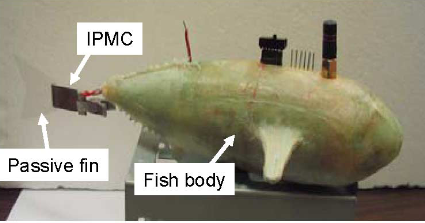
\includegraphics[width=0.7\linewidth]{ZhengRobot.png}%
	\caption{Робот рыбоподобной формы с хвостовым плавником в качестве движителя}
	\label{ZhengRobot}
\end{figure}

В работе~\cite{Wang_Tan} рассмотрен рыбоподобный робот, перемещающийся за счет периодического движения хвостового плавника (см. рисунок~\ref{WangRobot}). В прототипе робота хвостовой плавник изготовлен из углеволокна, который приводится в движение сервоприводом модели HS-5085MG фирмы Hitec. Плавник представляет собой пластину длиной 8 см, шириной 2.5 см и толщиной 1.1 мм. Движением сервопривода управляет микроконтроллер. В работе представлена модель движения, в основе которой лежит  динамика твердого тела и теория Лайтхилла, математически описывающая движение рыб~\cite{Lighthill_1970}. Основные уравнения движения записаны в виде уравнений Кирхгоффа для движения твердого тела в идеальной жидкости~\cite{Kirchhoff}, а теория Лайтхилла позволяет расчитать гидродинамические силы, действующие на подвижный хвостовой плавник. Проведены экспериментальные исследования по движению робота по окружности в бассейне при различном смещении начального угла хвостового плавника, а также с различной частотой колебания и амплитудой. При этом коэффициенты вязкого сопротивления и подъемной силы были аппроксимированы по модели используя экспериментальные данные при движении по окружности с параметрами начального смещения хвостового плавника в 20$^\circ$, частотой колебания $1.8\pi$ рад/с и амплитудой 15$^\circ$. Приведены графики на которых сравниваются результаты моделирования и экспериментов для радиуса окружности и времени ее прохождения. Далее получена зависимость коэффициентов вязкого сопротивления от начального смещения хвостового плавника, учитывая эти зависимости, отклонение полученных значений предыдущих экспериментов от расчетных уменьшилось. Затем проведены экспериментальные исследования движения робота по прямой. Модель с адаптированными коэффициентами вязкого сопротивления показывает также лучшее согласование с экспериментом чем модель с постоянными коэффициентами вязкого сопротивления.

\begin{figure}[h]
	\centering
	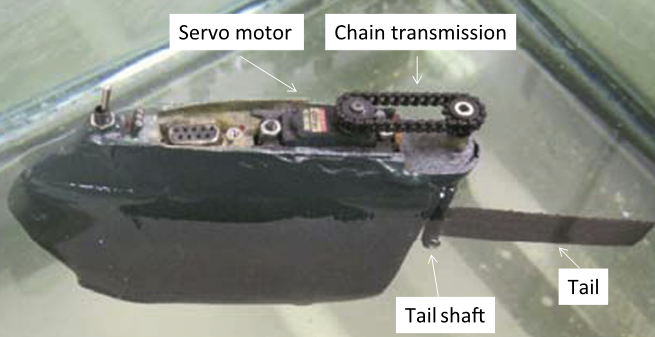
\includegraphics[width=0.7\linewidth]{WangRobot.png}%
	\caption{Рыбоподобный робот, перемещающийся за счет периодического движения хвостового плавника}
	\label{WangRobot}
\end{figure}

В работе~\cite{Zhou_2011} рассматривается мобильный водный робот движущийся в воде за счет колебаний боковых плавников (см. рисунок~\ref{ZhouRobot}). Такой способ управления имитирует движение ската. Робот имеет размеры 500 х 105 х 960 мм и массу 7.3 кг. Скорость движения робота 0.4 м/с. Плавники приводятся в движение сервоприводами по три на каждый плавник. Плавники изготовлен из эластичного резинового материала, по которому идут жесткие ребра от каждого сервопривода. Глубина погружения изменяется с помощью двунаправленного насоса, который может набирать воду во внутреннюю полость робота. Контролируется глубина датчиком давления. Законы управления роботом формируются используя модель нелинейного осцилятора Хопфа. В экспериментальных исследований представлены движения по прямой с поворотом. В будущем планируется ввести обратные связи для повышения эффективности управления.

\begin{figure}[h]
	\centering
	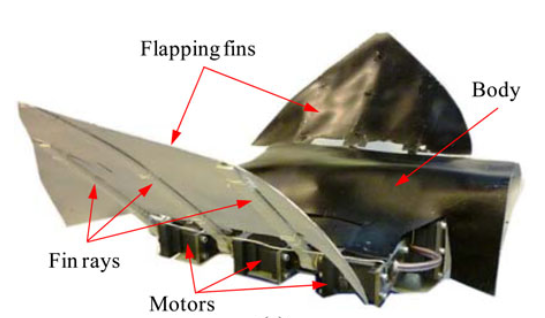
\includegraphics[width=0.7\linewidth]{ZhouRobot.png}%
	\caption{Мобильный водный робот, имитирующий движение ската}
	\label{ZhouRobot}
\end{figure}

\subsection{Перемещение за счет реактивной тяги}\label{sec:ch1/sec4}

Существуют конструкции, которые реализуют перемещение в жидкости реактивным методом. Движущая сила создается потоком воды, выталкиваемом из движителя, который, в основном, состоит из трубопровода, винта (насоса) и реверсивно-рулевого устройства. Данный тип движителя применялся на речных судах начиная с 50-х годов XX века. В настоящее время реактивные движителя применяются в небольших судах, плавающих на мелководье, начиная от моторных лодок и до скоростных судов.

В мобильной робототехнике реактивный тип движителя встречается нечасто. В качестве примера можно рассмотреть работу~\cite{Lin_2011}, в которой описан подводный робот сферической формы с водометными движителями (см. рисунок~\ref{LinRobot}). Робот имеет три реактивных движителя расположенные под углом 120$ ^\circ $ друг к другу. Каждый движитель имеет 2 степени свободы и может изменять направление выбрасываемой струи в горизонтальной и вертикальной плоскости. Проведены экспериментальные исследования, которые подтвердили возможность движения, используя простые маневры: движение в горизонтальной и вертикальной плоскостях, вращение вокруг вертикальной оси.

\begin{figure}[h]
	\centering
	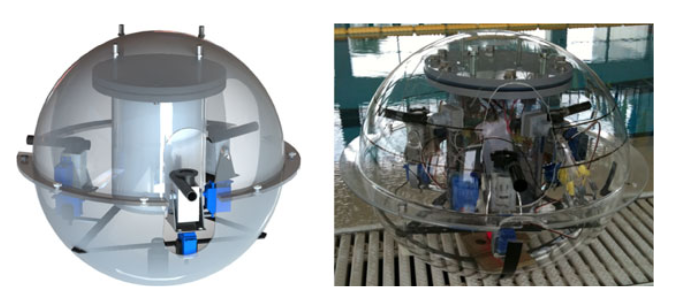
\includegraphics[width=0.7\linewidth]{LinRobot.png}%
	\caption{Подводный сфероробот с реактивными движителями}
	\label{LinRobot}
\end{figure}

\subsection{Перемещение за счет внутренних механизмов}\label{sec:ch1/sec5}

Устройства, перемещающиеся за счет движения внутренних масс так же представляют интерес. Можно подобрать необходимые характеристики движения внутренних масс для движения мобильного робота в заданном направлении. Отсутствие внешних подвижных элементов является главным преимуществом таких систем, так как воздействие на окружающую среду оказывается минимальное. Для исследования подобных объектов необходима математическая модель движения, которая поможет определить основные параметры и характеристики прототипа мобильного робота, а также необходимые условия для проведения экспериментов.

Для описания управляемого движения твердых тел в жидкости были предложены различные математические модели. Наиболее простые модели основаны построены в рамках теории идеальной жидкости и учитывают только эффект присоединенных масс. Однако такие существенно упрощенные модели позволяют обнаружить интересные динамические эффекты и закономерности, наблюдаемые в экспериментах. Например, в работах \cite{Kozlov_Ramodanov_PMM_2001, Kozlov_Onichenko} рассматривалось продвижение твердых тел в идеальной жидкости за счет подвижных внутренних масс. Было показано, что неограниченное продвижение оказывается возможным только при наличии анизотропии присоединенных масс. Идеи работ \cite{Kozlov_Ramodanov_PMM_2001, Kozlov_Onichenko} получили развитие в \cite{Vetchanin_Kilin_2016}, где рассматривалось движение эллиптического профиля, содержащего два эксцентрика, вращающихся в одинаковыми по модулю и противоположными по знаку скоростями. Было показано, что такая система движется в среднем прямолинейно. Данный факт подтверждается экспериментально, см. \cite{Klenov_Kilin_2016}. Также отметим работу \cite{Jing_Kanso_2013}, где рассматривалась задача устойчивости движения эллиптического профиля за счет вращательных колебаний. Трехмерные задачи управления и стабилизации движения эллипсоидов и винтовых тел рассматривались, например, в работах \cite{Borisov_et_al_2017, Vetchanin_Mamaev_2017, Vetchanin_et_al_2016, Woolsey_Leonard_1999}.

Модель схода вихрей позволяет описать самопродвижение тела за счет колебаний внутреннего ротора, наблюдаемое в экспериментах \cite{Tallapragada_2015, Pollard_Tallapragada_2019}. Однако, следует отметить, что сход каждого вихря приводит к увеличению размерности фазового пространства системы, что влечет определенные вычислительные трудности. Альтернативой описанной модели являются конечномерные математические модели, учитывающие вязкое трение и изменение циркуляции. Например, в работе \cite{Borisov_et_al_2018} рассматривалось плоскопараллельное движение эллиптического профиля за счет колеблющегося ротора при наличии периодически изменяющейся циркуляции и вязкого трения. Подобная модель для тела с острой кромкой и циркуляцией, изменяющейся согласно условию Кутты-Чаплыгина, была предложена в работе \cite{Mamaev_Vetchanin_2018} на основе результатов численных экспериментов, описанных в работе \cite{Mamaev_et_al_2018}. В работе \cite{Kilin_et_al_2018} была предложена модель движения робота с двумя эксцентриками, учитывающая помимо вязкого сопротивления, качку во время движения.

Отметим, что наиболее полное описание движения тел в жидкости может быть получено на основе совместного решения уравнений движения тела и уравнений Навье-Стокса, см., например, работы \cite{Childress_et_al_2011, Eldredge_2006, Vetchanin_et_al_2013}. Однако использование такого подхода затратно с вычислительной точки зрения при исследовании управляемого движения и построении гейтов. Поэтому моделирование с использованием уравнений Навье-Стокса целесообразно только при построении конечномерных моделей движения тел в жидкости, которые оказывают более удобными при анализе управляемого движения.

Рассмотрим более подробно некоторые работы.

В работе \cite{Volkova_Jatsun} рассматривается робот, состоящий из корпуса и двух по-движных внутренних масс, которые перемещаются относительно корпуса по прямолинейным направляющим (см. рисунок~\ref{JatsunRobot}). Взаимодействие робота со средой осуществляется только за счет четырех опорных поплавков с изменяемым углом наклона относительно вертикали. Движение происходит за счет изменения силы трения вдоль продольной оси корпуса при повороте поплавков. В той же работе приведена математическая модель и дается численное моделирование, позволившее изучить управляемые движения робота на примере прямолинейного и вращательного движения.

\begin{figure}[h]
	\centering
	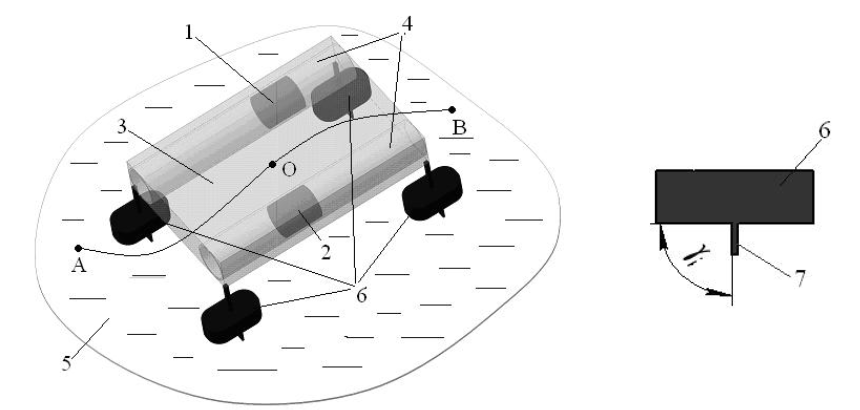
\includegraphics[width=0.7\linewidth]{JatsunRobot.png}%
	\caption{Схематичное изображение плавающего робота и схема поплавка}
	\label{JatsunRobot}
\end{figure}

В диссертации~\cite{Klenov_diss} и в работе~\cite{Klenov_Kilin_2016} рассмотрена локомоционная мобильная платформа, перемещающаяся в жидкости за счет изменения распределения масс (см. рисунок~\ref{TolikRobot}). Разработана математическая модель плоскопараллельного движения для идеальной жидкости и математическая модель движения с учетом внешних сил, действующих на объект со стороны жидкости на основе уравнений Кирхгоффа~\cite{Kirchhoff}. Первая математическая модель показала только качественное согласование результатов моделирования и экспериментов, тогда как вторая, уточненная модель движения, позволила достичь количественного согласования. В работах описана конструкция изготовленного натурного образца~\cite{patent_BNR}, который движется по поверхности жидкости. Проведены и описаны экспериментальные исследования. 

\begin{figure}[h]
	\centering
	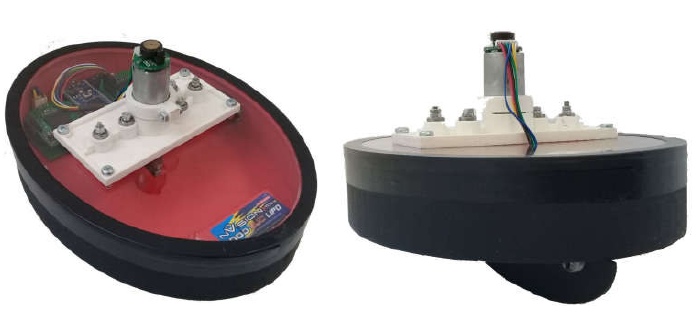
\includegraphics[width=0.7\linewidth]{TolikRobot.png}%
	\caption{Локомоционная мобильная платформа, перемещающаяся в жидкости за счет изменения распределения масс}
	\label{TolikRobot}
\end{figure}

В работе~\cite{Tallapragada_2015} рассмотрен водный робот, имеющий форму профиля крыла NACA 0030 (см. рисунок~\ref{TallapragadaRobot}). Робот перемещается в жидкости за счет периодического вращения внутреннего ротора. Разработана математическая модель движения, учитывающая сход вихрей с острой кромки. Проведены экспериментальные исследования. 

\begin{figure}[h]
	\centering
	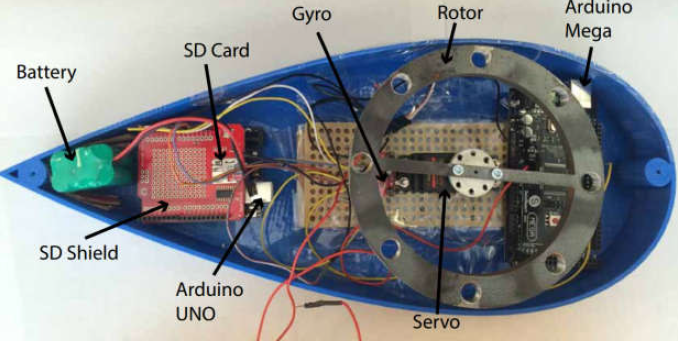
\includegraphics[width=0.7\linewidth]{TallapragadaRobot.png}%
	\caption{Водный робот, имеющий форму профиля крыла NACA 0030}
	\label{TallapragadaRobot}
\end{figure}

А в работе~\cite{Pollard_Tallapragada_2019} проведено сравнение маневренности вышеописанного робота при различных вариантах исполнения хвостовой части корпуса: полностью жесткий корпус, корпус со свободно вращающимся однозвенным хвостом, два варианта корпуса со свободно вращающимся двузвенным хвостом (см. рисунок~\ref{TallapragadaRobot2}).

\begin{figure}[h]
	\centering
	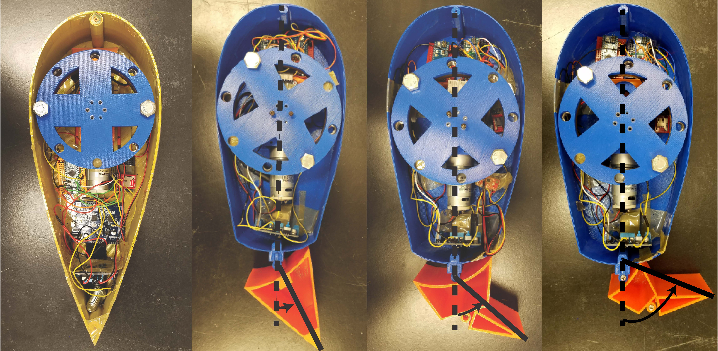
\includegraphics[width=0.7\linewidth]{TallapragadaRobot2.png}%
	\caption{Варианты исполнения водного робота со свободно вращающимся хвостом}
	\label{TallapragadaRobot2}
\end{figure}



В работе \cite{Ramodanov_Tenenev} рассматривается задача о движении тела в вязкой жидкости, за счет перемещения внутренних масс, при котором внешняя оболочка тела остается неизменной. Приведена математическая модель, построенная на гидродинамических уравнениях Навье-Стокса. В результате численного моделирования показано существенное влияние сил и момента вязкого сопротивления на траекторию движения, выявлены отличия движения тела в вязкой жидкости по сравнению с идеальной. На основе полученных результатов в работе \cite{Vetchanin_Tenenev_2011} решена задача оптимального управления движением тела по заданной траектории за счет перемещения внутренних масс, с применением гибридного генетического алгоритма. В результате получены аппроксимационные зависимости для сил, действующих на тело.

Исследование характеристик движения тела с переменным распределением массы в трехмерной вязкой жидкости проведено в работе \cite{Vetchanin_Mamaev_Tenenev_ND_2012}, а в работе \cite{Kilin_Vetchanin_DAN_2016} рассмотрено управляемое движение при наличии циркуляции вокруг тела. В этих работах показана возможность перемещения тела в произвольном направлении, а также возможность преодоления силы тяжести телом с плавучестью близкой к нулевой.





